\hypertarget{triangulation-and-structured-light}{%
\section{Triangulation and Structured
Light}\label{triangulation-and-structured-light}}

The last section explored using time of flight to determine the distance
traveled. Distances can also be determined by using geometric properties
of the object (or image of the object). The approach is to project a
well defined light pattern (points, lines) onto the environment and
objects within. The reflected light is then captured by a
photo-sensitive line or matrix (camera) sensor device. Simple
triangulation then allows the computation of the distance in question.

Kinect and ASUS sensors use arrays of projected IR dots. The size of the
dot indicates distance of the dot. If the size of object is known, then
triangulation can be done without projecting light. Standard computer
vision techniques can recover relative image size.

\begin{quote}
Laser Triangulation.
\end{quote}

Laser Triangulation is done by setting the measurement apparatus up so
that simple trigonometry can be used to measure distance,
\texttt{lasertriangulation}. In this case, the laser setup uses similar
triangles making the mathematics much simpler. The distance \(D\) is
given by

\[D = \displaystyle\frac{fL}{x}.\]

All sensing involves error. We will address types of errors and how to
mitigate errors in the chapter on filtering. To get a feel for how
errors affect a result, one can run a simple numerical experiment.
Compute the range of the input values based on the error. Plug the high
and low values in and you can compute the range on the output value. The
following example provides some details.

\textbf{Example}

Assume that for the triangulation setup in \texttt{lasertriangulation},
we have \(f=8\)mm, \(L = 3\)cm and \(x = 2\)mm. Using the formula we see
that \(D = 0.8*3/0.2 =12\)cm. What if there is error in the \(x\) or
\(L\) measurement?

What is the error in the distance if we know that \(x\) has a max of
20\% error? A 20\% variation means that our value ranges between
\([1.6, 2.4]\). We can plug the two values in and see what the range in
D is. This works because \(D\) is a monotonic function of both \(x\) and
\(L\)\footnote{Monotonic means that \$f'\textgreater0\$ or
  \$f'\textless0\$ in the interval of interest.} Plugging these values
in we have \(10 \leq D \leq 15\). Which gives \(15/12 - 1 = 0.25\) or
25\% error. If we have 10\% error in \(L\), it gives
\(10.8 \leq D \leq 13.2\) or a 10\% error off of \(12\). To combine
these, we look for the largest and smallest values possible for \(D\),
given the range in input values. For \(x=1.6\) and \(L=3.3\) we get
\(D=16.5\). Likewise for \(x=2.4\) and \(L=2.7\) we get \(D=9\). The max
of the two is a 37.5\% error (from \(D=12\)cm).

Is there a way to estimate combined error from the equation? In
Calculus, the total derivative for \(f(x,y,z)\) :

\[df = \frac{\partial f}{\partial x}  dx + \frac{\partial f}{\partial y} dy + \frac{\partial f}{\partial z} dz\]

can be used to gain an error formula:

\[E = \Delta f \approx \frac{\partial f}{\partial x} \Delta x + \frac{\partial f}{\partial y} \Delta y + \frac{\partial f}{\partial z} \Delta z .\]

Using the values from the last example, \(f=8\)mm, \(L = 3\)cm and
\(x = 2\)mm and the variations, \(x\) has a max of 20\% error and 10\%
error in \(L\), find the error estimate for \(D\). Using
\(\Delta L = \pm 0.3\), \(\Delta x = \pm 0.04\), and variation in \(f\)
means \(\Delta f = 0\) we have

\[E  = \frac{L}{x} \Delta f +  \frac{f}{x} \Delta L - \frac{fL}{x^2} \Delta x
    = \frac{3}{0.2} (0) +  \frac{0.8}{0.2} (\pm 0.3) - \frac{(0.8)(3)}{(0.2)^2}(\pm 0.04)
    = \pm 3.6\]

This estimates an error of 25\%. This turns out to be not so accurate. A
20\% error is a bit too large for the linear approximation to be close,
but works as a rough estimate.

A way to modify the previous laser distance example is a common
industrial vision setup. Look at the diagram and see what formulas can
we derive. Note that:

\[\left(\frac{z}{x}\right) = \left(\frac{f}{u}\right) \qquad \mbox{and}\quad\tan(\alpha) = \left( \frac{z}{b-x} \right)\]

Flip the second formula:

\[\cot(\alpha) = \left(\frac{b-x}{z}\right)\]

Then multiply by z:

\[\left( z \right)\cot(\alpha) = \left( b-x \right)\]

Move the \(x\) over:

\[\left( z \right)\cot(\alpha) + x = b\]

From the first ratio: \(z = \cfrac{fx}{u}\).

\begin{quote}
Computer Vision
\end{quote}

Plug this in for \(z\):

\[\left(\cfrac{fx}{u}\right)\cot(\alpha) +x  = b.\]

Factor out the \(x\) and divide the rest over:

\[x = \frac{b}{\left(\frac{f}{u}\right)\cot(\alpha) + 1}\]

then using

\[z = \cfrac{fx}{u} = \left(\frac{f}{u}\right)\frac{bu}{\left(\frac{f}{u}\right)
\cot(\alpha) + 1} .\]

Summarizing the formulas:

\[x = \frac{b u}{f\cot \alpha + u},  \quad
z = \frac{b f}{f\cot \alpha + u}\]

What are \(x\) and \(z\) if b = 20cm, f = 2cm, \(\alpha\) = 60deg, and u
= 7mm? So, using these formulas:

\[x = 20*0.7/(2\cot(60)+0.7) = 7.55 cm,\]

\[z =
20*2/(2\cot(60)+0.7) = 21.57 cm.\]

The Sharp distance sensor uses a very similar approach to estimate
distances. The displacement of the beam center on the beam detector is
used for the distance estimate, see \texttt{fig:SharpIRsensor}. Distance
D is given by

\[D=  \frac{fb}{2d} .\]

Because the focal length is small, the range of distances are limited by
the resolution of the detector (which provides \(D\)). The Sharp
detector returns the distance estimate as an analog voltage. An analog
to digital converter can be used to provide the numerical value. In
practice, the relation between voltage and distance is not linear and
some calibration in software is required.

\begin{quote}
Sensor package.
\end{quote}

\begin{figure}
\centering
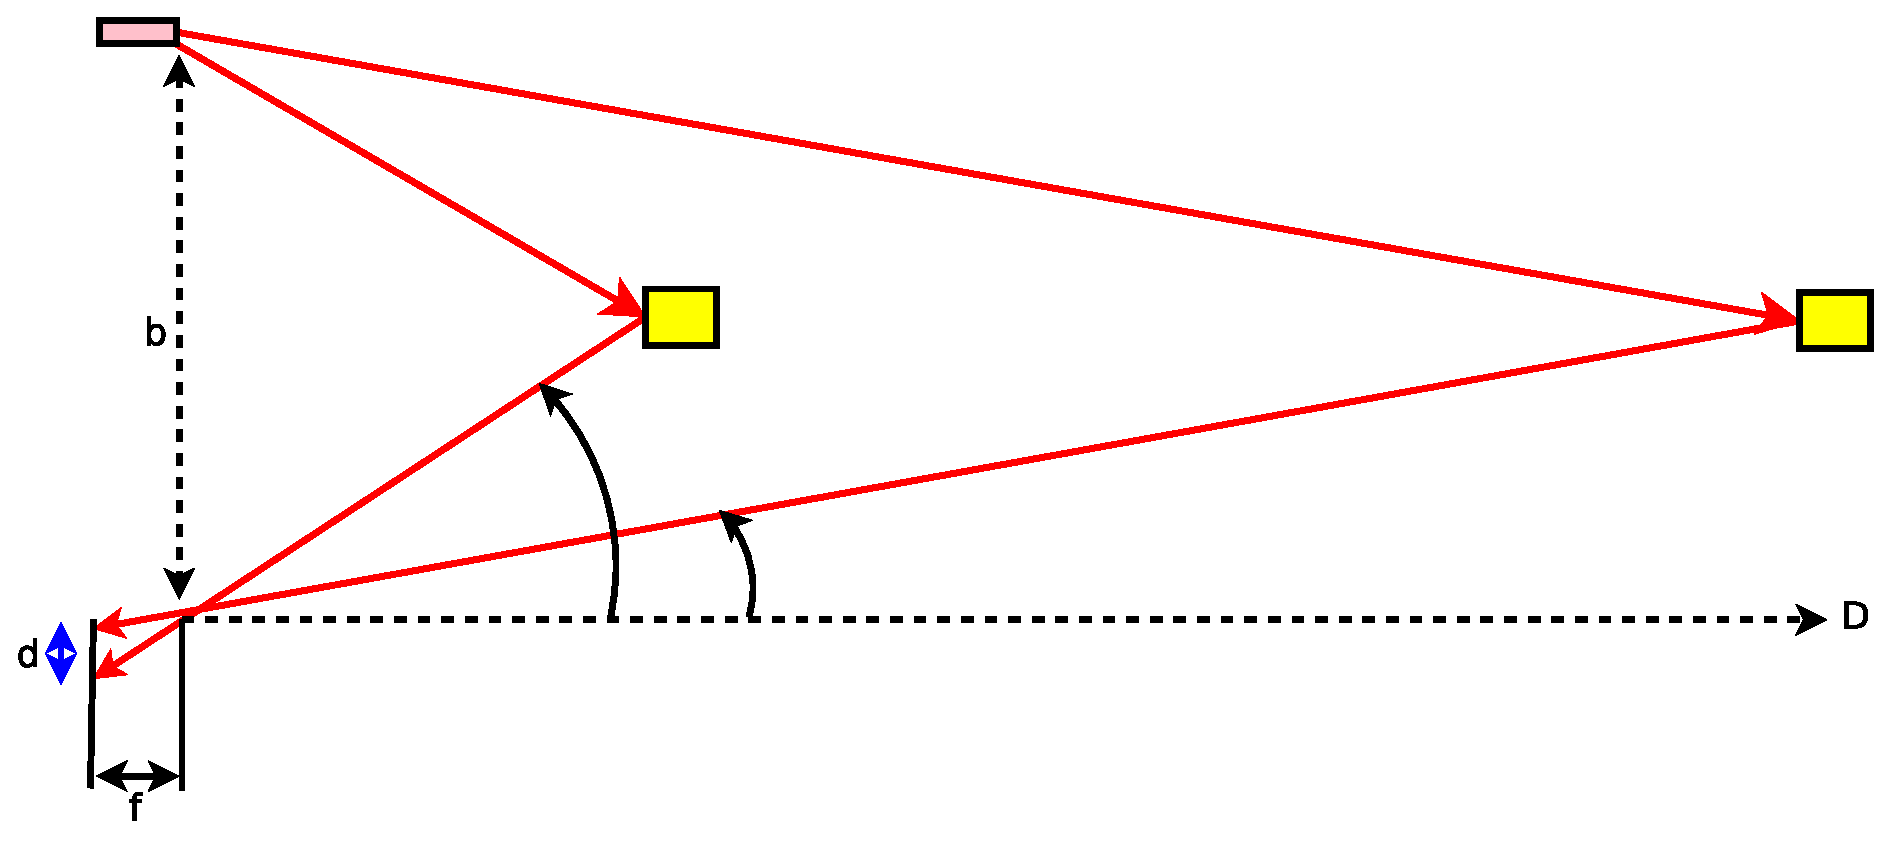
\includegraphics[width=0.7\textwidth,height=\textheight]{SensorsFigures/sharp.*}
\caption{The triangulation used to calculate distance}
\end{figure}

Another approach used in machine vision is \textbf{Structured Light}. A
known pattern of light is projected onto the environment. Common
patterns are dots, stripes and grids. A camera will view the
instrumented scene and determine the object heights using geometry.

\begin{quote}
Structured light.
\end{quote}

\textbf{Footnotes}
